%%%%%%%% ICML 2019 EXAMPLE LATEX SUBMISSION FILE %%%%%%%%%%%%%%%%%

\documentclass{article}

% Recommended, but optional, packages for figures and better typesetting:
\usepackage{microtype}
\usepackage{graphicx}
\usepackage{subfigure}
\usepackage{booktabs} % for professional tables

% hyperref makes hyperlinks in the resulting PDF.
% If your build breaks (sometimes temporarily if a hyperlink spans a page)
% please comment out the following usepackage line and replace
% \usepackage{icml2019} with \usepackage[nohyperref]{icml2019} above.
\usepackage{hyperref}

% Attempt to make hyperref and algorithmic work together better:
\newcommand{\theHalgorithm}{\arabic{algorithm}}

% Use the following line for the initial blind version submitted for review:
%\usepackage{icml2019}

% If accepted, instead use the following line for the camera-ready submission:
\usepackage[accepted]{icml2019}

% The \icmltitle you define below is probably too long as a header.
% Therefore, a short form for the running title is supplied here:
\icmltitlerunning{MIT 6.862 Applied Machine Learning Project Report}

\usepackage{amsmath}
\DeclareMathOperator*{\argmin}{arg\,min}


\begin{document}
	
	\twocolumn[
	\icmltitle{\normalsize MIT 6.862 Applied Machine Learning Project Report \\ \Large A Comparison between Machine Learning and Deep Learning for Cancer Diagnostics}
	
	% It is OKAY to include author information, even for blind
	% submissions: the style file will automatically remove it for you
	% unless you've provided the [accepted] option to the icml2019
	% package.
	
	% List of affiliations: The first argument should be a (short)
	% identifier you will use later to specify author affiliations
	% Academic affiliations should list Department, University, City, Region, Country
	% Industry affiliations should list Company, City, Region, Country
	
	% You can specify symbols, otherwise they are numbered in order.
	% Ideally, you should not use this facility. Affiliations will be numbered
	% in order of appearance and this is the preferred way.
	\icmlsetsymbol{equal}{*}
	
	\begin{icmlauthorlist}
		\icmlauthor{Matthew West}{hsph}
	\end{icmlauthorlist}
	
	\icmlaffiliation{hsph}{Department of Biostatistics, Harvard T.H. Chan School of Public Health, Boston, Massachusetts, United States}
	
	\icmlcorrespondingauthor{Matthew West}{mwest@hsph.harvard.edu, mjwest@mit.edu}
	
	% You may provide any keywords that you
	% find helpful for describing your paper; these are used to populate
	% the "keywords" metadata in the PDF but will not be shown in the document
	\icmlkeywords{Machine Learning, ICML}
	
	\vskip 0.3in
	]
	
	% this must go after the closing bracket ] following \twocolumn[ ...
	
	% This command actually creates the footnote in the first column
	% listing the affiliations and the copyright notice.
	% The command takes one argument, which is text to display at the start of the footnote.
	% The \icmlEqualContribution command is standard text for equal contribution.
	% Remove it (just {}) if you do not need this facility.
	
	\printAffiliationsAndNotice{}  % leave blank if no need to mention equal contribution
	%\printAffiliationsAndNotice{\icmlEqualContribution} % otherwise use the standard text.
	
	%\fontsize{11}{13}\selectfont
	\begin{abstract}
		This project presents a comparison between traditional machine learning on the structured Wisconsin Breast Cancer dataset and deep learning approaches to the corresponding raw images from which this dataset was derived. Classifiers for the structured data are determined and their cross-validated metrics reported, moving beyond accuracy to account for class imbalance and domain-specific requirements. Convolutional neural networks are trained on the raw images and transfer learning using ImageNet weights is shown to be effective in improving validation metrics over networks trained from scratch.
	\end{abstract}

	\section{Introduction and Related Work}
	Machine learning techniques are becoming increasingly commonplace across many domains, and medical
	diagnostics is no exception. Increasingly, classification and regression techniques are being applied
	to waveform analysis, image analysis, and electronic health records, to aid in clinical prediction and diagnostics \cite{panch2018artificial}. Among the many concerns that arise in applying machine learning to healthcare are the
	reliability and accuracy of classifiers used to aid human medical professionals in diagnostics. This provides the context for this project, which aims to assess issues related to the feasibility of using supervised learning for classification in this way, and in particular a comparison between traditional machine learning and deep learning for these purposes.
	
	%The particular set of challenges associated with deep learning in medical imaging in particular are an area of open research. Medical imaging tends to be interested in binary classification diagnostics whereas the bulk of computer vision appears to be large multi-class classification 
	
	In particular, this project concerns image classification on the Wisconsin Breast Cancer dataset, a set of images that depict cells from breast tumours, which are labeled either `malignant' or `benign', and which was accessed using the UC Irvine Machine Learning Repository \cite{Dua:2019}. This dataset first appeared in the early 1990s, and has received substantial attention since then \cite{street1993nuclear}. It is a structured dataset with features hand-computed from raw images. For this project, Professor Nick Street at the University of Iowa, one of the original authors of the work that introduced this dataset, kindly provided access to a set of the original raw images from which the structured dataset was derived. This allowed for a comparison between traditional machine learning on the structured dataset and deep learning applied to the raw images directly, which was identified as a key area of interest for this project.
	
	\section{Problem Setup}
	%This section presents a detailed description of the dataset, as well as a formal statement of the machine learning task at hand. 
	\subsection{Datasets}
	\subsubsection{Wisconsin Breast Cancer Dataset}
	The data used in this project is the Wisconsin Breast Cancer dataset, collected by a group at the University of Wisconsin-Madison. This structured dataset was derived from a set of fine-needle aspirate (FNA) images of breast tumour tissue, which is a method of imaging tumours that is relatively non-invasive compared to a full biopsy. Cellular regions within the image were segmented by hand and a set of summary statistics are computed for each cell within the image. Averages and extreme values of these features for cells across an image are then computed and used as features for classification.
	
	The dataset has 569 instances with 30 features, with 10 base features computed from the images: radius, texture, perimeter, area, smoothness, compactness, concavity, concave points, symmetry, and fractal dimension. The rest derive from these base features, with the mean, standard error and worst example being computed across the whole image, where `worst' is defined as the most clinically relevant indicator of malignancy for that feature. In addition to these features, each instance has an ID number and a label of `M' for malignant or `B' for benign. There are 212 malignant examples and 357 benign examples, and this imbalance has implications for classification. 
	\subsubsection{Raw Images - Data Wrangling}


	The set of raw images was obtained from an online repository provided by Professor Nick Street, each of which is an RGB image of dimensions 640 x 480 pixels \cite{NickStreetWebsite}. The relevant images were downloaded, and by processing their file names, it was possible to cross-reference each image with a corresponding ID in the Wisconsin Breast Cancer dataset, thus providing the appropriate labels. Of the 569 instances in the structured dataset, it was possible to identify corresponding raw images for 554 of them, with these examples being split between 206 malignant and 348 benign examples.
	
	\begin{figure}[b]
		\vskip 0.2in
		\begin{center}
			\centerline{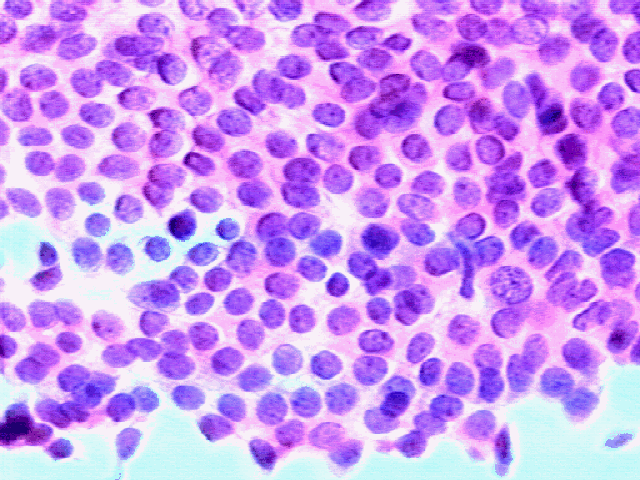
\includegraphics[width=0.4\columnwidth]{S_85_7373}\hspace{0.5em}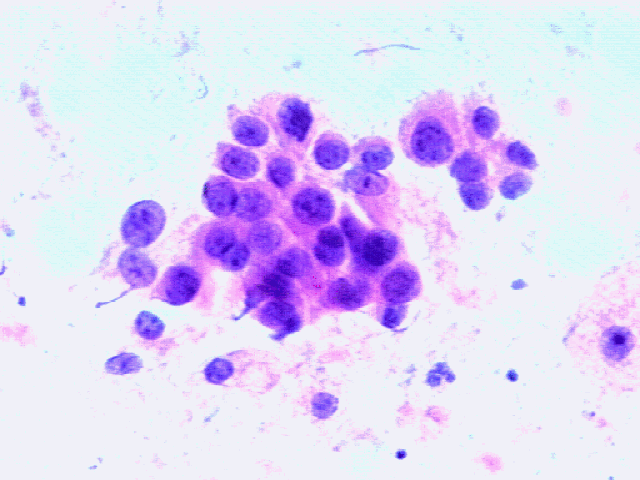
\includegraphics[width=0.4\columnwidth]{S_87_12729}}
			\caption{Two raw fine-needle aspirate images of breast tissue from which features were computed. The left-hand example is benign and the right-hand example is malignant.}
			\label{raw-image}
		\end{center}
		\vskip -0.2in
	\end{figure}
	
	\subsection{Model and Training}
	The task at hand is binary classification between the two classes, malignant and benign. We denote the hypothesis learned by an algorithm as $h(x^{(i)}; \theta)$, where $x^{(i)}$ is an instance in our dataset, and $\theta$ is a learned parameter or vector of parameters that parameterizes a decision boundary between the two classes. Here, $i$ is an index that denotes the $i^{th}$ pair, $(x^{(i)}, y^{(i)})$, where $i \in \{1,...,n\}$, with $n$ being the number of pairs in our dataset. Our dataset $\mathcal{D}$ is the set of $n$ pairs of examples $x^{(i)}$ and their corresponding labels $y^{(i)}$. Each label $y^{(i)}$ is binary, with malignant examples being encoded as 1, and benign as 0. $x^{(i)}$ either corresponds to a 30-dimensional vector of features or a raw image of shape \texttt{(480,640,3)} to be processed via convolution in a convolutional neural network. The loss function used throughout will be that of binary cross-entropy, with regularization terms included depending on the specifics of the algorithm. The objective of classification is to learn $\theta$ such that the loss is minimized on the training data, which can be stated formally as
	
	\begin{equation}\label{objective}
	\theta = \underset{\theta}{\argmin} \; \frac{1}{n}\sum_{i=1}^{n} L\left(h(x^{(i)}; \theta), y^{(i)}\right),
	\end{equation}
	
	where $L(h(x^{(i)}; \theta), y^{(i)})$ is the loss function describing how far the predicted label given by the hypothesis is from the training label. For this problem, it is binary cross-entropy, and if our prediction is denoted by $\hat{y}^{(i)} = h(x^{(i)}; \theta)$, then the loss function $L(\hat{y}^{(i)}, y^{(i)})$ is given as
	
	\begin{equation}\label{bin-cross}
	-y^{(i)} \log \hat{y}^{(i)} - (1 - y^{(i)}) \log (1 - \hat{y}^{(i)})
	\end{equation}
	
	where $\log$ is the natural logarithm.
	
	The performance of any particular classifier will then be evaluated for the given algorithm or hyperparameter using 5-fold cross-validation, subject to metrics like accuracy, precision, and recall. Note also that regularization terms can be added to the objective given by equation (\ref{objective}), though the presence of this term and its analytical form will be specific to the algorithm, and so is not included here.
	
	\section{Experimental Methods and Results}
	\subsection{Traditional Machine Learning Methods}
	The first subject of investigation was to look at traditional machine learning methods on the structured Wisconsin Breast Cancer dataset. A number of candidate algorithms were identified and compared in the first part of this project, and they are presented again here with additional parameter tuning and alternative metrics. These algorithms were logistic regression, a generalized linear model which is a natural algorithm for binary classification, (Gaussian) naive Bayes, a linear classifier that assumes independence between all features, and the XGBoost classifier, a gradient boosting algorithm that can learn nonlinear decision boundaries and constitutes the only ensemble method used in the analysis. All algorithms were implemented using Python 3 and the packages scikit-learn and XGBoost, and all of them were validated using the scikit-learn API \cite{scikit-learn, chen2016xgboost}. All models were run in a Google Colaboratory notebook with an Nvidia Tesla P100 GPU backend.
	
	Stratified 5-fold cross-validation was used throughout, and accuracy was used initially for cross-validation purposes. However, it was noted that accuracy is not the most appropriate metric given the imbalance between positive and negative examples in the dataset, and so this investigation included consideration of precision, recall, and the $F_{1}$ score. In the context of medical imaging, false positives are less of an issue compared to false negatives, as it is more important to detect disease if it exists, and so recall is the more important metric. However, optimising on recall alone could lead to predicting all cases as malignant, and so a good compromise is to use the $F_1$ score, which is the harmonic mean of precision and recall. The use of the $F_1$ was thus selected as the metric of choice when tuning hyperparameters.
	
	\begin{table}[t]
		\caption{Cross-validated classification metrics for naive Bayes, logistic regression, and the XGBoost classifier. All values for metrics are scaled to be percentages. Any hyperparameters that were tuned during the validation process are included in the bottom row. For naive Bayes, this was \texttt{var\_smoothing}, the fraction of the largest variance of any feature that is added to the other variances for numerical stability. For XGBoost, $\lambda$ is \texttt{lambda\_reg}, the hyperparameter governing L2 regularization, and $n$ is \texttt{n\_estimators}, the number of trees to fit. For logistic regression, $C$ is equivalent to the inverse of $\lambda$ in L2 regularization. Only those hyperparameters mentioned were tuned, with any others left as their defaults.}
		\label{ML-table}
		\vskip 0.15in
		\begin{center}
			\begin{small}
				\begin{sc}
					\begin{tabular}{lcccr}
						\toprule
						 & Naive Bayes & Logistic & XGBoost \\
						&(Gaussian)&Regression\\
						\midrule
						Accuracy    & 94.2$\pm$ 2.3& 96.6$\pm$ 1.8& 97.5$\pm$ 1.7\\
						Precision 	& 94.3$\pm$ 2.1& 96.7$\pm$ 2.1& 98.5$\pm$ 1.9\\
						Recall    	& 90.1$\pm$ 4.6& 94.3$\pm$ 3.2& 94.7$\pm$ 2.4\\
						$F_{1}$    	& 92.1$\pm$ 3.0& 95.5$\pm$ 2.3& 96.6$\pm$ 2.0\\
						Hyper-     	& \tiny\texttt{var\_smoothing} & $C = 1000$& $\lambda = 0.27$\\
						parameters  & \small= \texttt{1e-09}&&$n=1000$\\
						\bottomrule
					\end{tabular}
				\end{sc}
			\end{small}
		\end{center}
		\vskip -0.1in
	\end{table}
	
	
	As is evident from Table \ref{ML-table}, the XGBoost classifier was the preferred algorithm for learning, and performed the best across all metrics, being the only classifier to beat the benchmark of 97.3\% accuracy set in the original paper. This is not surprising as it can learn a non-linear boundary, and is an ensemble method that can average over several boosted trees. Logistic regression also performed well, on account of the inclusion of a regularization term in the loss function, whereas no parametric regularization was included for the naive Bayes classifier. Details regarding the relevant hyperparameters are also given in Table \ref{ML-table}.

	\subsection{Raw Image Dataset - Deep Learning}
	\subsubsection{Convolutional Neural Networks}
	Having explored traditional machine learning methods on the structured dataset, it was decided to investigate the implementation of classification on the raw image data. Before going down this route it was apparent that the due to the low quantity of labeled data available, that it would be difficult to train a neural network of sufficient complexity to both fit to the training data and to generalize to the validation set. Regardless, it was decided to explore a variety of architectures and see how comparable the cross-validated results could get to those in Table \ref{ML-table}. 
	
	Convolutional neural networks are used widely in image classification, and have few parameters and so are faster to train than fully connected dense networks. The convolutional layers, often followed by a pooling layer, have the property of picking up features in an image in a translation-invariant manner, which fits exactly with the classification problem at hand. In computing the features for the raw dataset, segmentation was done manually and features were derived based on geometric properties from individual cells within an image that typically contained several cells. Many derived features, such as those derived features defined by being the `worst' within an image would rely on this property of translational invariance which therefore offers a clear motivation for using convolutional layers in this classifier.
	
	All models were implemented using the package Keras, using a TensorFlow backend. \cite{chollet2015keras}.  As before, all models were run in a Google Colaboratory notebook with Nvidia Tesla P100 GPU hardware accelerator.
	
	The first challenge was finding an architecture that could be trained to fit to the training data, which proved difficult due to the small amount of data available. Following this, the architecture that performed the best on the specified validation metrics was determined and is depicted in Fig. \ref{small-cnn}. 5-fold cross validation was again used and, as predicted, cross-validation metrics showed the classifier did not generalize well to new data (See Table 
	\ref{CNN-table}). 
	
	\begin{figure}[]
		\vskip 0.2in
		\begin{center}
			\centerline{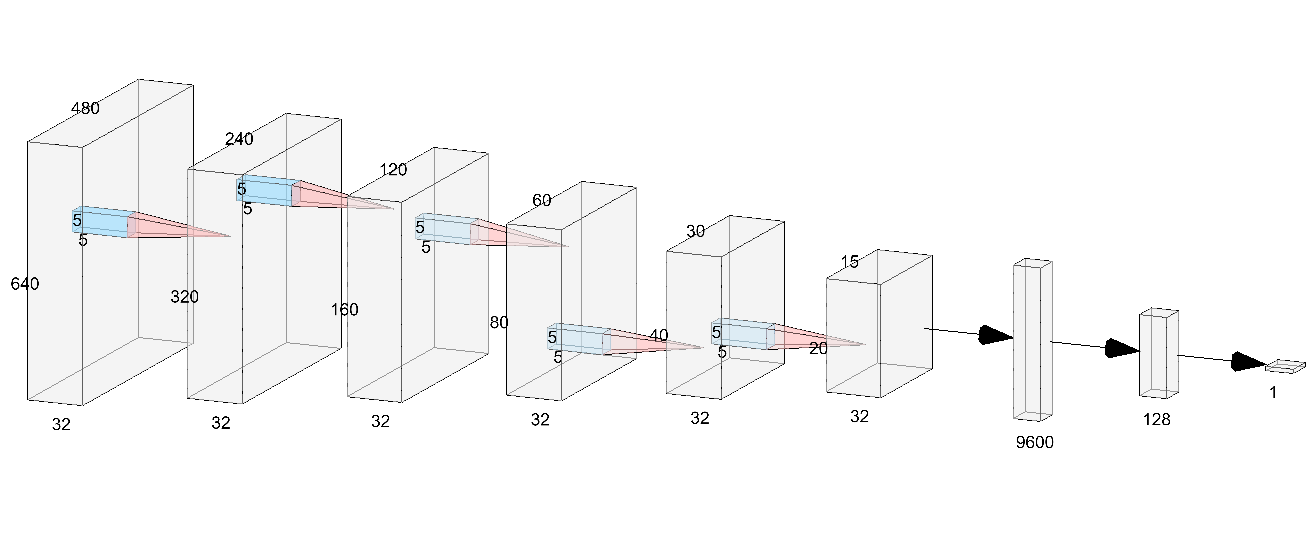
\includegraphics[width=\columnwidth]{Archi2}}
			\caption{Small CNN architecture trained from scratch. Each box corresponds to 32 5x5 filters being applied in a convolutional layer, using a ReLU activation and `same' padding, followed by a 2x2 max-pooling layer (not shown). The total number of trained parameters is 1,334,017. This output is flattened and then passed to a fully-connected layer with 128 units and a ReLU activation, to a single unit with sigmoid activation for class probability.}
			\label{small-cnn}
		\end{center}
		\vskip -0.2in
	\end{figure}
	
	\subsubsection{Transfer Learning}
	Having successfully fit the raw image data to a CNN and predictably reaching a roadblock in terms of performance on validation data, it was decided to explore transfer learning on the set of images. This involves using a large pre-trained neural network to serve as the basis for either weight initialization, or a frozen forward pass that is ignored at training time but can serve as a feature set for a new set of layers which ar trained on top of it. 
	
	As before, Keras was used to train all models. A number of deep architectures were imported from Keras, all trained on ImageNet data and with the final dense classification layers removed. VGG16 and VGG19 were the two architectures that were chosen to perform classification, and their results are summarized in Table \ref{CNN-table}. On top of these networks, a \texttt{Conv2D()} layer was added with filter size 3x3 and depth 32, followed by a 2x2 \texttt{MaxPooling2D()} layer. A dense layer was added with ReLU activation, with 256 and 512 units for VGG16 and VGG19, respectively. The output of this layer was output to a single unit with sigmoid activation, as previously. The VGG16-based architecture performed best across all metrics, including recall and $F_1$.
	
		\begin{table}[t]
		\caption{Cross-validated classification metrics for convolutional neural networks, both and using transfer learning. All values for metrics are scaled to be percentages. In each case, binary cross-entropy loss was used with stochastic gradient descent used for optimization with the default Keras hyperparameters.}
		\label{CNN-table}
		\vskip 0.15in
		\begin{center}
			\begin{small}
				\begin{sc}
					\begin{tabular}{lcccr}
						\toprule
						& Small & Transfer & Transfer \\
						&CNN&VGG16&VGG19\\
						\midrule
						Accuracy    & 69.3$\pm$ 2.5& 87.9$\pm$ 2.7& 85.2$\pm$ 3.0\\
						Precision 	& 59.1$\pm$ 4.6& 82.9$\pm$ 3.7& 77.3$\pm$ 1.8\\
						Recall    	& 49.9$\pm$ 6.9& 78.9$\pm$ 8.4& 77.4$\pm$ 6.7\\
						$F_{1}$    	& 52.8$\pm$ 5.1& 79.9$\pm$ 5.1& 76.6$\pm$ 3.7\\
						\bottomrule
					\end{tabular}
				\end{sc}
			\end{small}
		\end{center}
		\vskip -0.1in
	\end{table}
	
	
	\section{Discussion}
	With both the traditional machine learning and deep learning investigations yielding results in line with expectations, it would of course be better to continue this analysis with more data, particularly for the CNN investigation. In the repository Professor Street provided access to, there were many more images available, but without corresponding labels for supervised learning. This could allow for this image dataset to be expanded, or else for a semi-supervised learning approach to be employed, incorporating those images without labels. Another approach to improving generalization would be data augmentation, which was not explored in depth here.
	
	Results from transfer learning were promising with noticeable improvements over small CNN's trained from scratch. A paper in proceedings at NeurIPS 2019 addresses the use of transfer learning in medical imaging specifically and notes that for datasets much larger than the ones considered here, transfer learning provides lackluster performance gains in a medical imaging context \cite{raghu2019transfusion}. It is suggested that this may be due to these architectures being optimized for multi-class image classification benchmarks like ImageNet and may not provide useful features for medical diagnostics. This corresponds to their finding that feature re-use was largely confined to the earlier layers, which are likely to contain more abstract features. At the input end, too, ImageNet images are much smaller than the high resolution images typically seen in medical diagnostics, with downsampling required for their use in existing deep architectures used for transfer learning. This suggests that transfer learning applications that are trained for more specific domains will have to become more common if they are to see use beyond the realm of ImageNet-type problems. 
	
	The introduction of benchmark datasets for medical imaging problems would encourage research in this field and would likely provide significantly more relevant feature sets for researchers and clinicians with access to modestly-sized datasets hoping to apply transfer learning to their problems. Until then, this gap remains to be filled with researchers in other domains relying on architectures optimized for ImageNet.	
	
	\section{Conclusion}
	An investigation of traditional machine learning on an established structured dataset has been presented alongside a more experimental investigation of CNN's for image classification. Classification was successful on the structured dataset, meeting the target benchmark set in the original paper from which it was derived, and extending this to more domain-specific metrics. Transfer learning has been successfully applied to classification on raw images, and a number of potential improvements for further improving transfer learning-based approaches in medical imaging have been identified.
	
	
	
	% Acknowledgements should only appear in the accepted version.
	\section*{Acknowledgements}
	
	I would like to acknowledge Professor Nick Street at the University of Iowa for the original study and for providing access to the raw data, as well as for his helpful correspondence. Additionally, I would like to acknowledge Belén C. Saldías Fuentes and Ferran Alet at MIT for helpful feedback and Haoxin Li at Harvard for inspiration in the early stages of the project. 
	
	% In the unusual situation where you want a paper to appear in the
	% references without citing it in the main text, use \nocite
	%\nocite{langley00}
	
	\bibliography{example_paper}
	\bibliographystyle{icml2019}
	
	
\end{document}


% This document was modified from the file originally made available by
% Pat Langley and Andrea Danyluk for ICML-2K. This version was created
% by Iain Murray in 2018, and modified by Alexandre Bouchard in
% 2019. Previous contributors include Dan Roy, Lise Getoor and Tobias
% Scheffer, which was slightly modified from the 2010 version by
% Thorsten Joachims & Johannes Fuernkranz, slightly modified from the
% 2009 version by Kiri Wagstaff and Sam Roweis's 2008 version, which is
% slightly modified from Prasad Tadepalli's 2007 version which is a
% lightly changed version of the previous year's version by Andrew
% Moore, which was in turn edited from those of Kristian Kersting and
% Codrina Lauth. Alex Smola contributed to the algorithmic style files.
